\documentclass[
    a4paper,
    ngerman,
    11pt
]{scrartcl}
%   options include 12pt or 11pt or 10pt
%   classes include article, report, book, letter, thesis


\usepackage[T1]{fontenc}
\usepackage{lmodern}
\usepackage[utf8]{inputenc}
\usepackage[]{babel}

% for pictures
\usepackage{graphicx}
\usepackage{caption}
\usepackage{subcaption}
\usepackage{epstopdf}

% for citing urls correctly 
\usepackage{url}
\usepackage{hyperref}

\usepackage{listings}
\lstdefinestyle{customc}{
  belowcaptionskip=1\baselineskip,
  breaklines=true,
  frame=L,
  xleftmargin=\parindent,
  language=Python,
  showstringspaces=false,
  basicstyle=\footnotesize\ttfamily,
  keywordstyle=\bfseries\color{green!40!black},
  commentstyle=\itshape\color{purple!40!black},
  identifierstyle=\color{black},
  stringstyle=\color{blue},
}
\lstset{style=customc}

\usepackage[space]{grffile}
\usepackage{gensymb}
\usepackage{amsmath}
\usepackage{mathtools}
\usepackage{xfrac}
\usepackage[table]{xcolor}
\usepackage{tikz}

\title{Molekulare Motoren}
\author{Gruppe 26\\ Anh Tong \\ Tobias Theil \\ Kholodkov Jakov }
\date{\today}

% stands for the degree sign 
\newcommand{\dee}{{$^{\circ}$}} 	
\newcommand{\degr}{^{\circ}}
\newcommand{\shf}{$SF_6$}
\newcommand{\abs}[1]{\ensuremath{\left\vert#1\right\vert}}

\begin{document}
	
\maketitle
\tableofcontents
\bibliography{literatur}
\bibliographystyle{unsrt}

\newpage
\section{Einleitung}


%%% Local Variables:
%%% mode: latex
%%% TeX-master: "../motors.tex"
%%% End:
\section{Verwendete Methoden}

\section{Funktionsweise des flouriszierenden Aktinmarkers}
Für die Messung der Aktingeschwindigkeit wurde ein floursizierender Marker verwendet.
Floureszenz beschreibt eine spezielle Art der Abstrahlung von
Photonen durch einen quantenmechanischen Positionswechel
eines Elektron in einen energetisch niedrigeren Zustand.
Für Floureszenz braucht es ein Dreiniveausystem. Indem man die passende Lichtfrequenz verwendet,
werden Elektronen in das höchste Energieniveau angeregt,
von dem sie sich schnell, ohne Photoemission, in das mittlere Niveau abregen.
In diesem Energieniveau verweilen sie, bis es spontan zu einer 
Abregung und der damit verbundenen Lichtemission kommt.
Da die Energiedifferenz zwischen mittlerem und niedrigstem Energieniveau kleiner ist als
die Energiediffernz zwischen dem niedrigsten und dem höchsten Niveau, ist die Wellenlänge
des abgestrahlten Lichtes kleiner. Das wird schematisch in Abbildung
\ref{fig:dreiniveausystem} verdeutlicht.

\begin{figure}[]
  \centering
  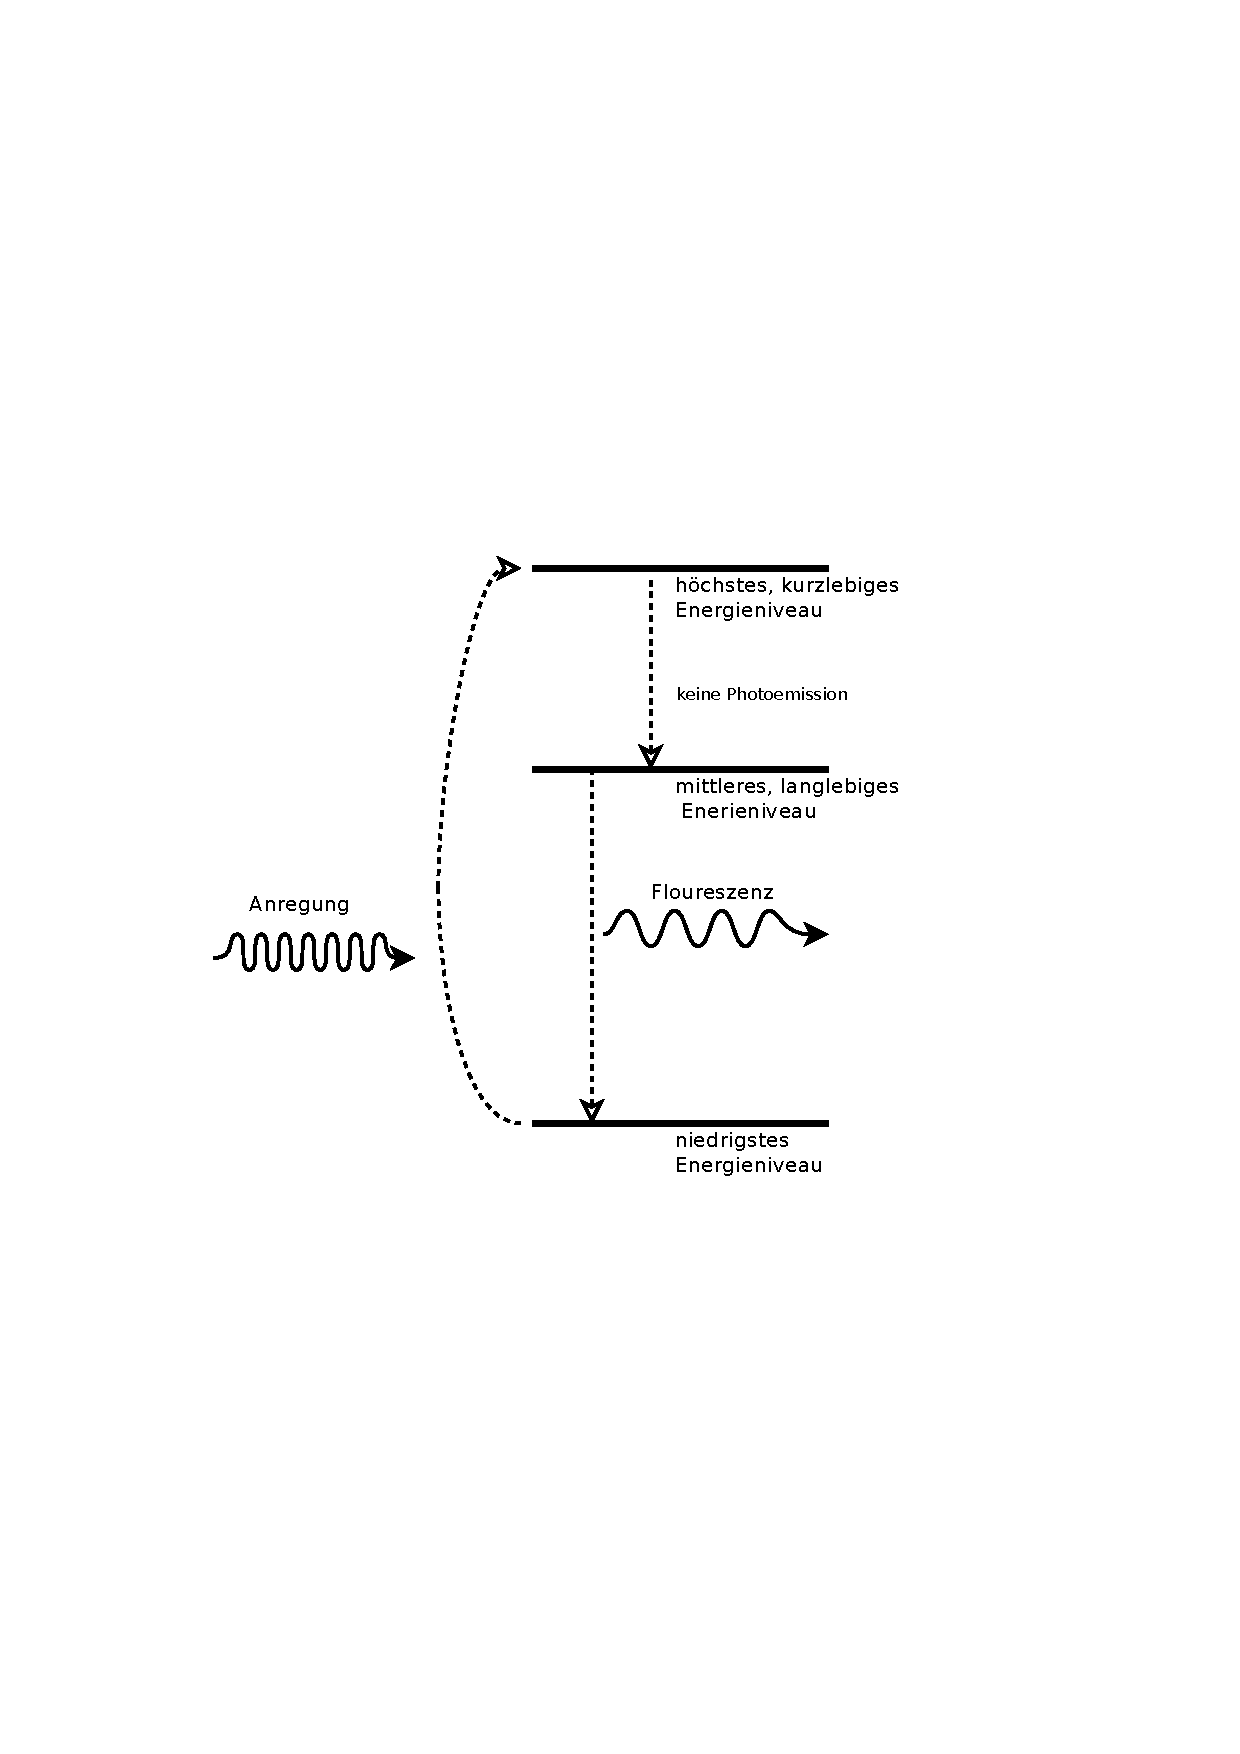
\includegraphics[width=\textwidth]{bilder/energieniveauschema.pdf}
  \caption{Ein Dreiniveausystem für Floureszenz}
  \label{fig:dreiniveausystem}
\end{figure}

\section{Zusammenhang zwischen numerischer Apertur und Auflösungsgrenze}
Um die Bewegung der Aktinfilamente in diesem Versuch zu beobachten, werden diese mit einem am Pilzgift Phalloidin gebundenen Farbstoff markiert.\\
Der hier zu beobachtende Effekt ist die Fluoreszenz. Atome fluoreszierender Stoffe werden durch Absorption von Photonen einer bestimmten Wellenlänge angeregt und beim Übergang in den Grundzustand wird ein Photon emittiert. In der Regel ist das emittierte Licht langwelliger als das eingestrahlte, dies lässt sich wie folgt erklären:\\
Bei der Anregung des Elektrons werden höhere Schwingungszustände des angeregten Zustands besetzt und ein Teil der Energie des anregenden Photons wird bei Schwingungsrelaxationen abgegeben. Zudem werden beim Zurückfallen des Elektrons in den Grundzustand auch zunächst höhere Schwingungszustände des Grundzustands besetzt. Diese Prozesse bedingen eine größere Wellenlänge des emittierten Lichts als die des absorbierten.\\
\\
Die Auflösung eines Objekts mithilfe eines Mikroskops wird zum einen von der Wellenlänge des bestrahlenden Lichts und zum anderen von der numerischen Apertur des benutzten Objektivs bestimmt. Strukturen, die kleiner sind als die verwendete Wellenlänge können nicht aufgelöst werden.\\
Die Auflösungsgrenze $d_{min}$ kann mit dem Rayleigh-Kriterium berechnet werden:
\begin{equation*}
d_{min}=\frac{1.22}{2}\cdot \frac{\lambda}{NA}
\label{eq:floureszenz}
\end{equation*}
\\
Näherungsweise gilt $d_{min} \approx \frac{ \lambda}{N_{A}}$.\\
Stände in diesem Versuch ein Auf - oder Druchlichtmikroskop
für die Analyse der Aktingeschwindigkeit zur Verfügung, so ergäbe sich nach Gleichung (\ref{eq:floureszenz}) bei blauem
Licht mit $ \lambda = 488nm$ und der im Versuch gegebenen Linse eine
Auflösungsgrenze von 180 nm. \\
Die Auflösung des Floureszenzmikroskops beträgt $1.57 \sfrac{\mu m}{\text{Pixel}}$.
Bei einer Aktinlänge im Bereich von einigen $\mu m$ \cite{FOPRA_molecular_motors}
scheint die Auflösung eines gewöhnlichen Mikroskopes besser zu sein.
Jedoch würde man die Aktinstrukturen nicht erkennen, da es zu viel Streulicht gäbe.
So ist der Grund für die Verwendung eines Floureszenzmikroskopes der
deutlich bessere Kontrast des Floureszenzmikroskopes im Vergleich zum Auflicht-,
oder Durchlichtmikropskop.

%%% Local Variables:
%%% mode: latex
%%% TeX-master: "../motors"
%%% End:

\section{Experimentelles Vorgehen und Ergebnisse}
\subsection{whatever}


\begin{figure}[]
  \centering
  \includegraphics[width=0.8\textwidth]{bilder/g_strich.png}
  \caption{Linearer Fit von $g'$ über$(1-\beta)$}
  \label{fig:abbe}
\end{figure}



\section{Berechnung der Messunsicherheiten}
Für die Unsicherheit der ATP Stoffmengen wurde eine relative Unsicherheit
von 5\% durch Pippetierfehler angenommen. $N_{err} = 5 \%$
Bei der Ausmessung Aktingeschwindigkeit wurden mindestens 10 Aktinfasern gewählt,
die sich im Zeitintervall von 10 Sekunden durchgehend bewegt haben.
Aus den gemessenen Distanzen wurde der Mittelwert, und die Varianz bestimmt.
\[
  \text{Pixel}_{err} = \sqrt{\sigma} + 2
\]
Zu dem Distanzfehler noch der Auflösungsfehler des Mikroskops
von $2 \cdot \text{Pixellänge}$ aufaddiert. Der Faktor 2 kommt daher,
dass man am Anfang und am Ende der Aktinfaser den Fehler über eine Pixellänge hat.
\[
  v_{err} = \frac{\text{Pixel}_{err} \cdot \text{Pixellänge}}{10s}
\]
Die Pixellänge wurde uns mit $1.57\sfrac{\mu m}{\text{Pixel}}$ angegeben.
Der Zeitfehler wurde vernachlässigt.
Der lineare Fit nach Formel \ref{equ:michaelis_inverse} gibt die Fitparameter
$m = \sfrac{K_m}{v_{max}} \pm m_{err}$ und $t = \sfrac{1}{v_{max}} \pm t_{err}$ an.
\begin{equation}
	\sigma_{f(x_1,x_2,...)} = \sqrt{\sum\limits_{i=1}^n (\frac{\partial f}{\partial x_i} \cdot \sigma_{x_i})^2}
	\label{equ:staterr}
\end{equation}
Mit $K_m = \sfrac{m}{t}$ und $v_{max} = \sfrac{1}{t}$ und unter Verwendung der
gausschen Fehlerfortpflanzung \ref{equ:staterr} wurden die
Fehler des Fits mit
\[
  K_{m_{err}} = \sqrt{(\frac{m_{err}}{t})^2 + (\frac{m \cdot t_{err}}{t^2})^2}
\] 
\[
  v_{max_{err}} = \frac{t_{err}}{t^2}
\]
errechnet.
Ensprechend wurden die Fehlerwerte für die Fehlerbalken Berechnet.
Für die Berechnungen und das Plotten der Graphen wurde ein Pythonskript geschrieben.
Dieses kann auf der Webseite \url{https://github.com/JackTheEngineer/molecular_motors}
im Ordner \texttt{calc/} eingesehen werden.

%%% Local Variables:
%%% mode: latex
%%% TeX-master: "../motors.tex"
%%% End:

\section{Diskussion}

%%% Local Variables:
%%% mode: latex
%%% TeX-master: "../motors.tex"
%%% End:
 
\section{Weitere Anmerkung}
Aus dieser Arbeit haben wir als werdende Wissenschaftler die folgenden Lektionen gelernt:\newline
Man muss sehr präzise Arbeiten, denn bereits kleine Fehler wie beim Pippetieren können große Auswirkungen auf
das Messergebniss haben.
Zudem darf man Fits von Datenpunkten nicht blindlings vertrauen, da allein die eine unterschiedliche
Auftragunsart der Daten das Ergebniss deutlich ändern kann. Man sollte bei Punkten stets gewichtete Fits verwenden,
mit der Gewichtung $ w_i = \sfrac{1}{\Delta x_i^2}$.


%%% Local Variables:
%%% mode: latex
%%% TeX-master: "../motors.tex"
%%% End:


% Anhaege w
\begin{appendix}
\section{Anhang}
\subsection{Fragen}

\end{appendix}
 
\end{document}

%%% Local Variables:
%%% mode: latex
%%% TeX-master: t
%%% End:

